\documentclass[conference]{IEEEtran}
\IEEEoverridecommandlockouts
% The preceding line is only needed to identify funding in the first footnote. If that is unneeded, please comment it out.
\usepackage{cite}
\usepackage{amsmath,amssymb,amsfonts}
\usepackage{algorithmic}
\usepackage{graphicx}
\graphicspath{{./}{sections/}}
\usepackage{textcomp}
\usepackage{xcolor}
\usepackage{booktabs}
\usepackage{tabularx}
\usepackage{array}
\newcolumntype{C}[1]{>{\centering\arraybackslash}p{#1}}
\newcolumntype{Y}{>{\raggedright\arraybackslash}X}
\def\BibTeX{{\rm B\kern-.05em{\sc i\kern-.025em b}\kern-.08em
    T\kern-.1667em\lower.7ex\hbox{E}\kern-.125emX}}

% Use block-style subsubsections (heading on its own line)
\makeatletter
\renewcommand\subsubsection{\@startsection{subsubsection}{3}{\z@}%
  {0.75ex plus 0.2ex minus 0.1ex}%
  {0.25ex plus 0.1ex minus 0.1ex}%
  {\normalfont\normalsize\itshape}}
\makeatother
\begin{document}

\title{Computer-Use Agents: Ecological Landscape, Emerging Security Threats, and Future Governance Architecture\\
{\footnotesize \textsuperscript{*}Note: Sub-titles are not captured in Xplore and
should not be used}
\thanks{Identify applicable funding agency here. If none, delete this.}
}

\author{
\IEEEauthorblockN{Zejian Chen}
\IEEEauthorblockA{\textit{BUPT}}
\and
\IEEEauthorblockN{Zhanyuan Liu}
\IEEEauthorblockA{\textit{BUPT}}
\and
\IEEEauthorblockN{Xi Zhang}
\IEEEauthorblockA{\textit{BUPT}}
}

\maketitle

\begin{abstract}
This document is a model and instructions for \LaTeX.
This and the IEEEtran.cls file define the components of your paper [title, text, heads, etc.]. *CRITICAL: Do Not Use Symbols, Special Characters, Footnotes, 
or Math in Paper Title or Abstract.
\end{abstract}

\begin{IEEEkeywords}
component, formatting, style, styling, insert
\end{IEEEkeywords}

\section{Introduction}
\label{sec:introduction}

\emph{[Placeholder: Introduction to be completed.]}

\section{Background}

\subsection{From Content-Level Risks to Action-Level Hazards}

Conventional LLM systems are primarily exposed to \emph{content-level} failure
modes, including misleading generation, privacy-sensitive text leakage, and
overreaching recommendations. In these systems, harmful output is usually
bounded by language itself: the model ``says'' something wrong, unsafe, or
inappropriate. In contrast, Computer-Use Agents (CUAs) possess
environment-execution capabilities, allowing model outputs to be translated
into concrete operations across software interfaces. As a result, classical
LLM risks are not merely preserved but operationally amplified into
\emph{action-level} hazards with higher real-world impact.

\begin{itemize}
\item \textbf{Expanded input attack surface.} CUA perception is no longer limited
to a single prompt channel. Web pages, pop-up dialogs, emails, local
documents, chat messages, and desktop notifications can all function as
instruction carriers. This multi-channel exposure increases susceptibility to
indirect prompt injection, where malicious or irrelevant interface content
steers the agent away from user intent while appearing contextually
plausible [3--4, 16--18]. Unlike direct jailbreaking, these attacks are
embedded in ordinary task environments, making detection harder and
raising the likelihood of silent objective drift.

\item \textbf{Privilege and toolchain connectivity.} CUAs are often integrated
with persistent browser sessions, local file systems, terminal/script
execution, and authenticated account states. This creates a continuous path
from ``influence'' to ``execution'': an attacker-controlled instruction can
progress from content manipulation to privileged operations, such as data
exfiltration, unauthorized transaction steps, or unsafe command invocation
[4, 13--15, 33--36]. Therefore, the security boundary is no longer the model
response surface; it extends to every connected tool and credential context.

\item \textbf{Amplification in long-horizon workflows.} CUA tasks are frequently
multi-step, cross-application, and stateful. As horizon length grows, small
reasoning errors, permission mistakes, or policy violations can compound and
be automatically propagated across downstream actions. This temporal
amplification makes incidents more difficult to audit, attribute, and roll
back, especially when intermediate decisions are implicit or weakly logged
[26--31, 60--61]. Consequently, reliability and governance for CUAs must be
evaluated as process integrity over time, not only as single-turn response
quality.
\end{itemize}

Taken together, these properties indicate a categorical shift in risk: CUAs
should be modeled as socio-technical execution systems rather than text-only
assistants. This motivates security controls that combine prompt-level
defenses with runtime policy enforcement, least-privilege tool access,
action confirmation boundaries, and end-to-end traceability.

\subsection{Ecosystem-Specific Security: MCP and Skills}

Beyond generic CUA risks, two ecosystem components deserve explicit treatment:
\emph{MCP-based tool integration} and \emph{skill-based capability reuse}.
Both improve extensibility, but both also introduce additional trust
dependencies and compositional failure modes.

\textbf{MCP trust boundary risks.}
MCP-style integration allows an agent to access external tools/resources
through server endpoints. If endpoint identity, transport integrity, or tool
schema constraints are weak, a malicious (or compromised) MCP server can
inject manipulated outputs that appear operationally valid. This can convert
context poisoning into privileged side effects, including unauthorized file
access, leakage of sensitive workspace context, and hidden execution of unsafe
operations via abstract tool calls. In practice, MCP security is therefore not
only a connectivity issue; it is a cross-boundary execution integrity issue.

\textbf{Skill supply-chain and execution risks.}
Skills package prompts, scripts, and reusable workflows. This packaging model
reduces engineering overhead, but it creates plugin-like supply-chain risk.
Untrusted or poorly reviewed skills may contain over-privileged steps,
dangerous command templates, covert data egress logic, or prompt constructions
that degrade policy compliance. Even benign skills can become unsafe through
version drift and undocumented behavioral changes. Accordingly, skill adoption
requires provenance validation, version pinning, permission scoping, and
runtime policy checks rather than one-time functional testing.

\textbf{Compositional risk in long-horizon execution.}
The highest-impact failures often occur when skills orchestrate multi-step
actions across several MCP servers. Local checks may pass at each hop while
the end-to-end chain still violates user intent or security policy. This
visibility gap complicates accountability because different components may log
different abstractions of the same action. Hence, CUA assurance must evaluate
the entire execution graph (inputs, tool calls, credentials, state changes,
and side effects) under adversarial conditions, not isolated components.

\textbf{Governance implications.}
These properties motivate concrete controls in future CUA governance
architecture: authenticated MCP channels, strict tool I/O typing and policy
enforcement, least-privilege credential delegation, sandboxed skill execution,
high-risk action confirmation, and tamper-evident audit trails for incident
reconstruction. In short, MCP servers and skills should be treated as
first-class security principals, not neutral implementation details.
 

\section{Architecture}

\subsection{CUA Abstraction: A Closed-Loop Perception--Brain--Action System}

Modern Computer-Use Agents (CUAs) have evolved from early rule-based
heuristics into autonomous systems driven by multimodal large language models
(MLLMs). Synthesizing recent core studies, the foundational CUA framework can
be abstracted as a three-layer \emph{Perception--Brain--Action} (PBA)
architecture \cite{wang2024llm_agents_survey}. This architecture operates
across both GUI-centric and API-centric interaction pathways, while increasingly
coupling security mechanisms into the execution loop. The unified framework is
illustrated in Fig.~\ref{fig:cua_architecture}.

\begin{figure*}[t]
    \centering
    \includegraphics[width=\textwidth]{images/picture3.1.png}
    \caption{Three-stage CUA architecture under a closed-loop
    Perception--Brain--Action design. Stage 1 performs perception and
    sanitization, Stage 2 handles planning and reflection, and Stage 3 executes
    validated actions under sandboxed isolation.}
    \label{fig:cua_architecture}
\end{figure*}

\subsubsection{Perception: Alignment and State Representation in Heterogeneous Environments}

The perception layer transforms high-dimensional and noisy digital inputs (e.g.,
pixel streams, HTML sources, API responses) into structured state
representations consumable by foundation models. Technically, this layer has
shifted from metadata-dependent parsing to vision-native grounding.

\textbf{Structured text and DOM-based perception.}
Early web agents relied heavily on underlying interface metadata. WebArena and
Mind2Web used reduced DOM trees or accessibility trees as primary inputs
\cite{zhou2024webarena,deng2024mind2web}. While efficient in instrumented web
settings, such approaches are brittle in closed-source software and dynamic
rendering scenarios. In machine-centric interaction settings, Gorilla further
examined structured API-document and JSON-schema grounding for tool-use
decisions \cite{patil2023gorilla}.

\textbf{Pure visual grounding and multimodal localization.}
To remove dependence on privileged interface metadata, recent work moved toward
direct screenshot understanding. CogAgent and ScreenAI demonstrated that
high-resolution vision-language modeling can capture complex UI layout and
semantics \cite{hong2024cogagent,baechler2024screenai}. SeeClick and Ferret-UI
then introduced coordinate-grounded objectives, significantly improving
fine-grained element localization on desktop and mobile environments
\cite{cheng2024seeclick,you2024ferretui}. More recently, OmniParser proposed a
pure-vision parsing paradigm that tokenizes UI screenshots and extracts icon
semantics and text bounding boxes without external OCR dependency
\cite{lu2024omniparser}.

\textbf{Security-aware perception and environment sanitization.}
As CUAs are exposed to adversarial environments, perception-layer fragility has
become explicit. AgentXploit showed that hidden or context-poisoned interface
content can trigger indirect prompt injection and manipulate downstream agent
behavior \cite{liu2024agentxploit}. To mitigate this risk, Chen et al.
introduced visual pre-filtering and sanitization pipelines for VLM-based CUAs,
isolating untrusted external signals before they enter planning
\cite{chen2024defending_ipi_vlm}.

\subsubsection{Brain: Long-Horizon Planning, Memory, and Reflection}

The brain layer serves as the system's executive control module: it handles
goal decomposition, intent grounding, and dynamic routing across heterogeneous
action channels. Its central challenge is maintaining coherent reasoning under
long-horizon execution, where catastrophic forgetting and objective drift are
common.

\textbf{Temporal planning and dynamic routing.}
Building on the ReAct paradigm of interleaving reasoning and acting
\cite{yao2023react}, recent CUA systems adopt more explicit planning topology.
OSCopilot presented a general operating-system agent framework that decomposes
system-level objectives into executable subtasks \cite{wu2024oscopilot}. In
hybrid tool/UI settings, the brain must also perform cost-aware routing:
prefer direct API/tool invocations when available (Toolformer-style), and
degrade gracefully to GUI interaction when no reliable interface exists
\cite{schick2023toolformer}.

\textbf{Episodic memory and exploration.}
When operating in unfamiliar software environments, CUAs benefit from active
exploration and memory accumulation. AppAgent introduced autonomous trial-and-
error interaction to build episodic action--state memory for downstream reuse
\cite{zhan2024appagent}. AgentBoard evaluations further indicate that external
memory mechanisms (e.g., retrieval over trajectory traces) can improve success
rates in long-context, multi-turn tasks \cite{ma2024agentboard}.

\textbf{Closed-loop reflection and alignment guardrails.}
Real-world execution includes latency, UI non-determinism, and system errors.
Reflexion introduced verbal reinforcement and self-correction loops that allow
agents to backtrack and revise plans after failed actions \cite{shinn2023reflexion}.
To reduce long-horizon goal hijacking risk, recent secure-agent designs also
emphasize guardrails-by-construction, where side-channel monitors continuously
check whether decision trajectories remain aligned with user intent
\cite{liu2024agentxploit}.

\subsubsection{Action: Unified Action Space and Polyglot Sandbox Isolation}

The action layer compiles planned intent into concrete operational effects. Its
core design tension is balancing cross-platform generalization against
potentially destructive execution risk.

\textbf{End-to-end native GUI control.}
Traditional CUA stacks often depended on manually engineered controllers for
coordinate mapping and event translation. UI-TARS and follow-up systems
promoted an end-to-end paradigm that directly outputs absolute/relative
coordinates and keyboard/mouse events, reporting strong benchmark performance
\cite{qin2025uitars}. OS-ATLAS further showed that large-scale cross-platform
pretraining (Windows/macOS/Linux) can learn a more unified and generalizable
action space \cite{boyce2025osatlas}.

\textbf{Code-as-Action and Agent-Computer Interface (ACI).}
For backend-heavy or computation-intensive tasks, pure GUI clicking is often
inefficient. SWE-agent proposed an agent-computer interface (ACI) that allows
models to generate and execute Bash/Python code in terminal environments,
expanding CUA capability in software engineering workflows
\cite{yang2024sweagent}.

\textbf{Isolated execution and human-in-the-loop (HITL).}
Because action-layer outputs can directly mutate file systems, credentials, and
network states, environment-level isolation is critical. OSWorld and related
evaluation settings highlight the necessity of realistic yet controlled
execution environments \cite{xie2024osworld}. In production-grade deployments,
generated code should run in stateless containers or virtual machines; in
addition, sensitive operations (e.g., privilege escalation) should trigger
human-in-the-loop confirmation to provide strong validation for irreversible
actions.

\section{A Lifecycle Framework for Computer-Use Agents: From Capability Formation to Continual Adaptation}
\label{sec:lifecycle}

If Section~\ref{sec:architecture} explains what a CUA is made of internally, this section asks how those capabilities become operative in a real system. The comparative point of the lifecycle view is that similar runtime failures may reflect very different upstream causes, and similar design choices may become safe or unsafe depending on when they are introduced. More precisely, the tri-layer architecture offers a structural account of capability composition, whereas the lifecycle perspective explains how perceptual grounding, decision-making, and action execution are produced, bound to concrete platforms, stressed during use, and revised over time. The two views are therefore complementary: the architectural framework clarifies internal organization, while the lifecycle framework clarifies how that organization becomes a functioning, deployable, and governable agent in practice.

To capture this temporal and engineering dimension, we organize representative CUA research into four stages: \textit{Creation}, \textit{Deployment}, \textit{Operation}, and \textit{Maintenance}. This categorization should not be understood as a purely chronological decomposition of system development. Rather, it is motivated by a different analytical question: \emph{at what point in the lifecycle are capabilities formed, operationalized, stressed, and revised?} From this perspective, each stage identifies a distinct locus of capability formation, failure exposure, and safety intervention. Creation determines what perceptual and control priors an agent can acquire through data, model design, and training; Deployment governs how those capabilities are bound to interfaces, tools, permissions, and middleware; Operation tests whether the agent can sustain coherent behavior over long trajectories in open-ended environments; and Maintenance addresses whether the system remains reliable as interfaces drift, workflows change, and adversarial surfaces evolve. Although these stages are tightly coupled in practice and often iterated rather than traversed only once, they capture the dominant points at which CUA capability and risk are shaped across the full system lifecycle.

This shift matters analytically. Many failures that become visible during operation are rooted earlier in the lifecycle---for example, in the quality of grounding established during Creation or in the action abstractions and trust boundaries introduced during Deployment. Conversely, many apparent capability improvements matter only if they survive long-horizon operation and remain stable under post-deployment change. A lifecycle framework therefore does more than reorder prior work: it reveals where bottlenecks originate, where risks surface, and where evaluation and governance must intervene across the full trajectory of a deployed CUA.

\begin{figure*}[t]
\centering
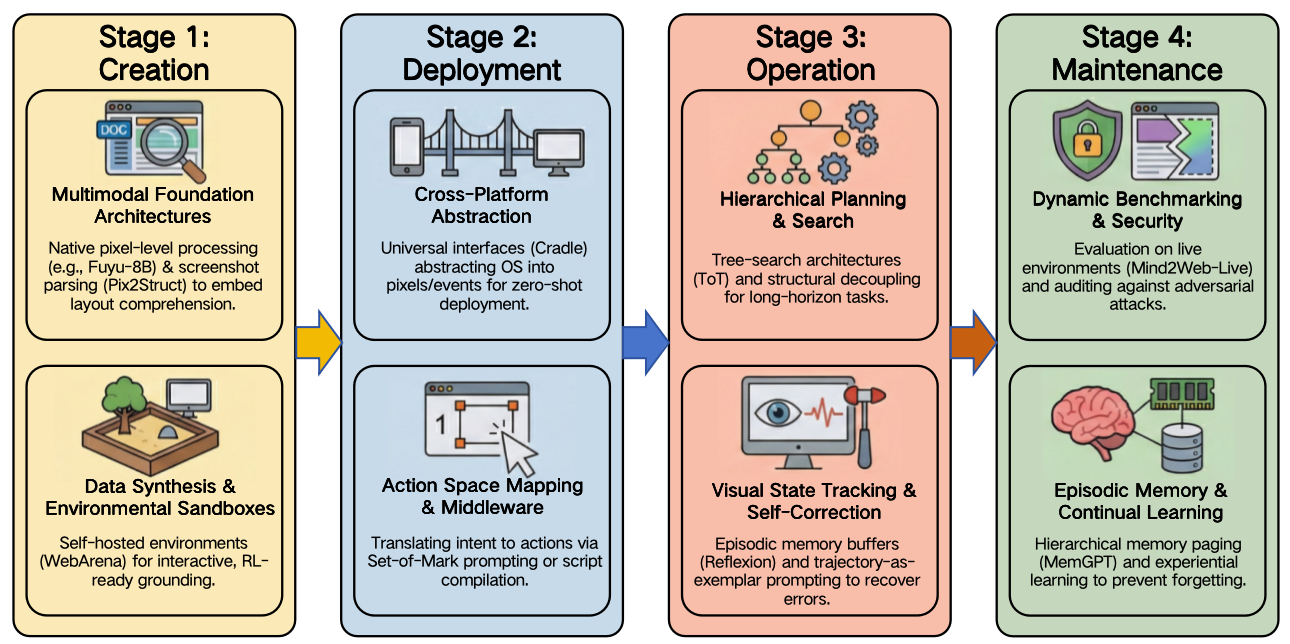
\includegraphics[width=\textwidth]{images/p4.1.png}
\caption{Four-stage lifecycle framework for CUAs: Creation, Deployment, Operation, and Maintenance. The stages correspond to capability formation, system binding, online stress, and continual adaptation.}
\label{fig:lifecycle_taxonomy}
\end{figure*}

\subsection{Creation Stage: Capability Formation Through Grounding, Data, and Training}

The Creation stage determines the \emph{capability ceiling} of a CUA before it interacts with a live environment. The key judgment in this stage is that many later robustness problems are not primarily runtime reasoning failures; they are inherited from what the system was taught to perceive, predict, and optimize. Its goal is not simply to scale model size, but to align \emph{semantic intent}, \emph{visual grounding}, and \emph{actionable interface structure} in ways that support downstream control. This stage is therefore most closely tied to the \emph{Perception Layer}: whether an agent can robustly interpret screens, localize interface elements, and distinguish task-relevant affordances is largely determined here.

Conceptually, Creation is analytically distinct because it is the stage at which usable control priors are \emph{acquired} rather than merely exercised. Accordingly, the most informative way to organize work at this stage is by the mechanisms through which actionable grounding is built: multimodal representation learning, trajectory and reward construction, and interactive training environments. These directions are not entirely separable in mature systems, but together they define the main routes through which pre-deployment capability is formed.

\paragraph{Multimodal grounding as the core bottleneck}
Earlier web agents relied heavily on structured states such as DOM trees, with methods like Mind2Web highlighting the need for filtering and task-centric distillation when raw interface representations become too large or noisy~\cite{deng2023mind2web}. Recent CUA research, however, increasingly treats GUI grounding as a first-class problem in its own right. CogAgent \cite{hong2024cogagent}, ScreenAI \cite{baechler2024screenai}, and SeeClick \cite{cheng2024seeclick} improved visual understanding and point-level action grounding, while newer systems such as WinClick \cite{hui2025winclick} show that pure screenshot-based grounding on desktop environments remains difficult without dedicated pretraining and benchmark design. The broader lesson is that creation-stage progress is no longer just about better multimodal encoders; it is about learning a stable mapping from heterogeneous visual interfaces to executable action semantics.

\paragraph{Data generation, reward design, and interactive training environments}
Recent work also shows that model quality is inseparable from the quality of trajectories, rewards, and environments used to train it. Classical datasets such as AITW \cite{rawles2023androidinthewild} and agent-tuning pipelines such as AgentTuning \cite{zeng2024agenttuning} established the importance of instruction-following trajectories, but they are increasingly complemented by more scalable and adaptive data sources. Open-foundation efforts such as OpenCUA \cite{wang2025opencua} extend this logic with large-scale demonstration capture, cross-OS task coverage, and end-to-end open CUA models. TongUI \cite{zhang2025tongui}, for example, converts multimodal web tutorials into large-scale GUI trajectories across platforms, while UI-R1 \cite{lu2025ui} and GUI-R1 \cite{luo2025gui} demonstrate that reinforcement learning with explicit action rewards can improve action prediction and generalization beyond pure supervised fine-tuning. Meanwhile, interactive environments such as WebArena \cite{zhou2023webarena} and OSWorld \cite{xie2024osworld} remain essential because they expose agents to non-stationary transitions, delayed consequences, and recovery behavior that static corpora cannot faithfully represent.

Overall, the Creation stage defines whether a CUA merely recognizes interface tokens or genuinely acquires \emph{actionable grounding}. It therefore sets the upper bound for downstream robustness. Many errors that later appear during operation---such as unstable localization, failure under visual ambiguity, or brittle transfer to unseen applications---often reflect representational or data limitations introduced at this stage rather than purely online reasoning failures.

\subsection{Deployment Stage: Binding Model Capability to Real Systems}
\label{sec:deployment}

If the Creation stage determines what a model can potentially understand, the Deployment stage determines how that capability is \emph{bound} to a real computing environment. The central comparative claim here is that deployment is where capability turns into authority, and it is often the stage that most directly sets the eventual blast radius of failure. This stage moves the problem from model construction to interface integration: observations must be attached to concrete platforms, and abstract action intent must be translated into executable control channels. Deployment is therefore not a passive implementation detail; it is where capability meets operating-system constraints, middleware, permissions, and platform heterogeneity.

Deployment forms a separate analytical stage because a capable model does not automatically become a usable agent. Between learned capability and real-world operation lies a system-binding problem: what interface is exposed, what actions are permitted, what middleware mediates intent, and what trust boundary surrounds execution. This is increasingly evident in open deployment systems illustrated by \textbf{OpenClaw}, whose public descriptions suggest a continuously reachable gateway that connects messaging channels, sessions, tools, and execution events into a shared control plane. In such systems, deployment is no longer merely a wrapper around a model; it is the stage at which user-facing communication surfaces, execution authority, and policy constraints are assembled into an operational agent stack.

For this reason, deployment work is most naturally organized by how it resolves the tension between broad portability and controlled actuation. In current CUA systems, this tension is most visible in two recurring design choices: whether to favor universal cross-platform interfaces or tighter environment-specific mediation, and how much semantic abstraction to insert between model output and executable action.

\paragraph{Universal interfaces and cross-platform abstraction}
A major design choice in deployment is whether to rely on platform-specific structure or system-agnostic control. Cradle \cite{tan2024cradle} exemplifies a universal philosophy by using screen pixels as input and keyboard/mouse events as output, enabling operation in visually rich environments without application-specific APIs. Related systems such as Mobile-Agent \cite{wang2024mobile}, OS-Copilot \cite{wu2024copilot}, and ScreenAgent \cite{niu2024screenagent} similarly emphasize broad deployability across mobile, desktop, and remote environments. Recent surveys of GUI and OS agents reinforce that such designs improve portability, but also increase dependence on strong visual grounding and low-level control stability~\cite{tang2025survey,hu2025agents}.

As publicly described, OpenClaw makes this deployment logic especially visible because the system is not tied to a single application surface. Instead, it appears as a multi-channel ingress layer spanning platforms such as WhatsApp, Telegram, Slack, Discord, and iMessage while remaining local-first in its control architecture. This kind of design expands portability in a deployment sense: the same agent can be reached across heterogeneous communication interfaces and remain continuously available beyond the workstation on which it runs. At the same time, it shifts more burden onto deployment-time policy design, since cross-channel exposure broadens the range of untrusted inputs, contextual ambiguity, and authority-routing decisions that the system must mediate.

\paragraph{Action abstraction, middleware, and trust boundaries}
Portability alone, however, does not guarantee reliable execution. A second line of work therefore introduces intermediate abstractions that reduce the gap between language-level intent and environment-level control. WebVoyager \cite{he2024webvoyager} uses Set-of-Mark prompting to simplify visual selection, OmniACT \cite{kapoor2024omniact} compiles decisions into executable scripts, and UFO \cite{zhang2025ufo} separates application selection from local action execution in desktop environments. These systems suggest that deployment success depends not only on \emph{where} an agent is mounted, but also on \emph{how} semantic intent is mediated before emission as low-level actions.

Deployment is also the stage where trust boundaries become concrete. In OpenClaw-like deployments, operators must make explicit decisions about which channels may reach the agent, which tools are enabled, whether sandboxing is applied, how sessions are isolated, and how network and automation settings are configured. These choices determine whether middleware acts as a safety-enforcing constraint layer or merely as a conduit for unconstrained execution. More broadly, deployment-time abstractions can either reduce downstream risk by narrowing action pathways and scoping authority, or amplify it by centralizing control while leaving permissions, extension points, and execution surfaces insufficiently separated.

Taken together, the Deployment stage is defined by a central trade-off between \emph{portability} and \emph{controllability}. System-agnostic interfaces generalize broadly, but they place heavier burdens on grounding and verification. More tightly integrated middleware can improve determinism and efficiency, but it introduces stronger assumptions about privileges, dependencies, and trusted execution channels. Publicly described open-deployment systems such as OpenClaw make this trade-off especially salient: once communication channels, tool invocation, session state, and system execution are bound through a single gateway layer, many failures that later appear as ``agent mistakes'' are in fact rooted in deployment-time decisions about abstraction, authority, and trust boundaries.
\subsection{Operation Stage: Long-Horizon Interaction, Memory, and Recovery}
\label{sec:operation}

Once deployed, a CUA enters the stage where its practical value is actually tested: live operation under changing interface states and real tasks. The main comparative result at this stage is that long-horizon reliability depends less on single-step plausibility than on memory discipline, verification, and recovery. At this point, the main challenge is no longer whether the agent can parse a screen or emit an action in principle, but whether it can maintain task coherence across long trajectories without drifting, looping, or compounding local mistakes. Accordingly, the Operation stage is where the \emph{Decision Layer} faces its greatest pressure.

Operation is analytically distinct because it is the point at which latent capability is exposed to real temporal stress. In this stage, failures are no longer hypothetical limitations of representation or interface binding; they become observable breakdowns in continuity, recovery, and control under non-stationary interaction. For this reason, the main axes of progress are best understood in terms of how systems sustain coherence online: by adding stronger execution structure, by preserving memory across steps, and by verifying whether previous actions actually produced the intended state changes.

\paragraph{From step-wise reaction to structured execution}
Earlier agent frameworks such as ReAct \cite{yao2022react} and Tree of Thoughts \cite{yao2023tree} established the value of explicit reasoning and search. In the CUA setting, however, recent work shows that planning must be combined with stronger execution structure. MobileUse \cite{li2025mobileuse} introduces hierarchical reflection to detect and recover from failures at multiple temporal scales, while WorldGUI \cite{zhao2025worldgui} demonstrates that current GUI agents degrade sharply under diverse initial states, revealing fragile long-horizon planning even when single-step actions appear plausible. ActionEngine \cite{zhong2026actionengine} pushes this trend further by shifting from reactive control toward programmatic execution based on an updatable GUI state-machine memory. Recent scaling results reinforce the same lesson from a different angle: Behavior Best-of-N improves OSWorld performance and generalizes to WindowsAgentArena and AndroidWorld by selecting among multiple rollouts through structured behavior narratives, suggesting that operational reliability depends on trajectory selection and verification rather than one-shot planning alone~\cite{gonzalez2025scalingcua}.

\paragraph{Memory, verification, and fault tolerance}
Recent literature also makes clear that long-horizon success depends not only on planning, but on runtime memory and post-action verification. Reflexion \cite{shinn2023reflexion} and Synapse \cite{zheng2023synapse} already suggested that agents benefit from self-feedback and experience reuse. More recent GUI-specific work sharpens this observation: execution failures increasingly stem from state loss, weak memory across steps, and the inability to verify whether prior actions had the intended effects. This is precisely why contemporary CUA research is moving toward structured memory, reflective recovery, and verifier-driven control rather than relying on a single monolithic prompt.

OpenClaw-like systems make this pressure especially concrete because persistent messaging channels and long-lived sessions compress multiple tasks, users, and contextual cues into the same runtime surface. In such deployments, weak memory scoping or inadequate post-action verification does not merely reduce benchmark accuracy; it can allow stale context, cross-task contamination, or ambiguous channel intent to persist across operational episodes.

The Operation stage is where local mistakes become global failures unless they are actively contained. Better planning, memory, and verification generally improve long-horizon robustness, but they also increase latency, context cost, and system complexity. The key challenge is therefore not merely to make agents more autonomous, but to make that autonomy \emph{stable} under environmental non-stationarity.

\subsection{Maintenance Stage: Continual Adaptation, Evaluation, and Security Hardening}
\label{sec:maintenance}

Unlike static benchmark models, CUAs operate in software ecosystems that evolve continuously. The main comparative lesson of the Maintenance stage is that post-release stability is itself an engineering variable: a strong system can decay quickly if evaluation, permissions, and ecosystem controls remain frozen while the environment changes. Interfaces are redesigned, workflows shift, permissions change, and adversarial surfaces emerge after deployment. For this reason, Maintenance should not be understood as a final cleanup stage after operation; it is the \emph{continual adaptation layer} that keeps the entire system valid over time.

Maintenance is best treated as a distinct stage because post-deployment validity is not guaranteed by one-time success at deployment or operation. Even a well-trained and initially well-behaved agent will degrade if the surrounding software ecosystem changes while its assumptions remain fixed. The core question of this stage is therefore how to preserve reliability under drift, shifting workflows, stale evaluation signals, and evolving attack surfaces. From this perspective, recent work can be read through three recurring maintenance functions: adaptation to interface and workflow change, continuous reliability evaluation, and post-deployment security hardening.

\paragraph{Adapting to UI drift and workflow change}
A first maintenance challenge is preserving capability under changing interfaces. Recent work shows that GUI failure is often caused not by complete task novelty, but by gradual visual and procedural drift. MAGNET \cite{sun2026magnet}, for example, explicitly addresses appearance drift and workflow drift through dual-level memory that separates stable functional semantics from evolving task procedures. This reframes maintenance as an ongoing problem of retaining invariant knowledge while updating interface-specific realizations.

\paragraph{Continuous evaluation and memory-aware reliability testing}
A second challenge is that static benchmarks quickly become stale in GUI environments. VisualWebArena \cite{koh2024visualwebarena}, WorkArena \cite{drouin2024workarena}, and Risky-Bench \cite{zheng2026riskybench} already move evaluation closer to realistic web, enterprise, and deployment-grounded settings, but recent evidence suggests that even these are not sufficient to characterize long-term reliability. MemGUI-Bench \cite{liu2026memgui} shows that existing mobile GUI benchmarks severely under-represent memory-intensive tasks and fail to assess cross-session learning, implying that maintenance requires continuous, capability-targeted evaluation rather than one-time benchmark success.

\paragraph{Security as a lifecycle maintenance problem}
Finally, maintenance must include post-deployment security hardening. Zero-Permission Manipulation \cite{qian2026zero} shows that GUI agents can be exploited through the observation-to-action gap, allowing malicious interfaces to rebind seemingly benign planned actions without requiring dangerous permissions. More recent deployment-facing studies make the same point in broader form: PASB \cite{wang2026pasb} reports vulnerabilities across prompt processing, tool usage, and memory retrieval in personalized OpenClaw scenarios, while Your Agent, Their Asset \cite{wang2026asset} shows that poisoning persistent capability, identity, or knowledge state can sharply raise attack success rates. ClawKeeper \cite{liu2026clawkeeper} responds with skill-, plugin-, and watcher-based protections intended to span multiple lifecycle stages. Together, these results suggest that some safety failures are not caused by poor reasoning alone, but by architectural assumptions that only become visible after deployment in dynamic environments. Maintenance must therefore include regression testing, attack-surface monitoring, and policy updates alongside model adaptation.

The same point extends to open ecosystems illustrated by public discussions around OpenClaw and Moltbook. Once tools, channel integrations, or agent communities evolve independently of the base model, maintenance must govern not only model quality but also ecosystem hygiene: version pinning, extension review, identity management, and policies for capability sharing become part of the reliability problem rather than optional platform administration~\cite{wang2026asset,liu2026clawkeeper}.

Taken together, the Maintenance stage reveals a final trade-off: continual updating improves adaptation and resilience, but it also increases evaluation overhead, regression risk, and governance complexity. Conversely, freezing a deployed system may preserve short-term stability, yet it leads to rapid decay once interfaces, workflows, or threat models change. For CUAs, maintenance is therefore not the last step in a linear pipeline; it is the mechanism that keeps the whole lifecycle operational.

\begin{table*}[!t]
\centering
\scriptsize
\caption{Illustrative mapping of OpenClaw-related deployment properties onto the master framework.}
\label{tab:openclaw_mapping}
\renewcommand{\arraystretch}{1.08}
\setlength{\tabcolsep}{3.5pt}
\begin{tabularx}{\textwidth}{L{2.75cm} L{1.8cm} L{2.8cm} Y}
\toprule
\textbf{Property} & \textbf{Location} & \textbf{Risk} & \textbf{Control} \\
\midrule
Persistent messaging ingress across channels~\cite{openclaw2026website,ibm2026openclaw} & Deployment & Mixed trust levels, ambiguous sender intent, broad ingress & Channel isolation, provenance tagging, session scoping \\
Local-first control plane bound to tools and sessions~\cite{openclaw2026website} & Deploy. + oper. & Concentrated authority, over-privilege, weak mediation & Least privilege, sandboxing, auditable mediation, approval for high-impact actions \\
Persistent sessions and carried-over runtime context & Operation & Cross-task contamination, stale context, verifier failure & Memory partitioning, expiry/reset policy, post-action verification \\
Agent-community or Moltbook-style capability exchange~\cite{chen2026openclaw} & Oper. + maint. & Capability diffusion, prompt propagation, ecosystem exposure & Signed exchange, identity/provenance preservation, registry discipline \\
\bottomrule
\end{tabularx}
\end{table*}

\subsection{Lifecycle Coupling and Analytical Implications}

The four stages above are analytically distinct but operationally coupled. Lifecycle analysis should therefore redirect attention from where failure is observed to where it becomes structurally likely: Creation determines the quality of grounding, Deployment defines the concrete interface and trust boundary, Operation tests long-horizon coherence, and Maintenance determines whether the overall coupling remains valid as environments and threats evolve.

This lifecycle view also sharpens the architectural framework introduced in Section~\ref{sec:architecture}. The \emph{Perception Layer} is primarily shaped during Creation, the \emph{Execution Layer} becomes operationally meaningful during Deployment, the \emph{Decision Layer} is most severely stressed during Operation, and Maintenance determines whether the coordination among all three layers remains stable over time. The lifecycle perspective therefore explains where CUA reliability and security are formed, exposed, and renegotiated.

\section{Security and Privacy Analysis}
\label{sec:security}

This section surveys the security and privacy risks associated with Computer-Use Agents (CUAs). Relative to conventional LLM safety, which has largely focused on dialogue behavior and text generation, CUA security must additionally account for \emph{action-level} risk: these systems perceive visual environments, interpret user goals, and execute low-level operations over external interfaces, thereby exposing vulnerabilities at the intersection of perception, reasoning, and execution~\cite{jones2025systematization,tian2023evil}. 

Following the lifecycle perspective introduced in Section~\ref{sec:lifecycle}, we organize the discussion according to the stages at which security and privacy failures are introduced, amplified, or realized. We first specify a threat model, then introduce an attribution framework that distinguishes model-subjective factors (curiosity and malice) from non-subjective environmental causes, and finally review representative threats across creation, deployment, execution, and maintenance. Table~\ref{tab:cua_threats} summarizes this taxonomy by lifecycle stage and attribution class. Because the survey is motivated in part by open deployment settings exemplified by OpenClaw, we place particular emphasis on risks that emerge when CUA capabilities are exposed through persistent communication channels, extensible tools, and long-lived execution contexts.

\begin{table*}[!t]
\centering
\small
\caption{Threat taxonomy by lifecycle stage and attribution (C: curious, M: malicious, E: environmental). Abbreviations: PoT, Plan-of-Thought; MCP, Model Context Protocol; TOCTOU, time-of-check to time-of-use; IPI, Indirect Prompt Injection; EIA, Environmental Injection Attack; RAG, Retrieval-Augmented Generation; PII, personally identifiable information.}
\label{tab:cua_threats}
\setlength{\tabcolsep}{5pt}
\renewcommand{\arraystretch}{1.15}
\begin{tabular}{>{\raggedright\arraybackslash}p{1.55cm}
                >{\raggedright\arraybackslash}p{4.2cm}
                >{\raggedright\arraybackslash}p{1.55cm}
                >{\raggedright\arraybackslash}p{8.1cm}}
\toprule
\textbf{Stage} & \textbf{Threat Type} & \textbf{Attribution} & \textbf{Representative Work} \\
\midrule
Creation & PoT backdoor, training-time poisoning & M & BadVLA~\cite{zhou2025badvla}, Hidden Ghost Hand~\cite{cheng2025hidden} \\
Creation & Unsafe action interfaces and safety gaps & E & OS-Harm~\cite{kuntz2025harm}, CUAHarm~\cite{tian2025measuring} \\
Deployment & Over-privilege, weak isolation & E & Jones~\cite{jones2025systematization}, CSAgent~\cite{gong2025secure} \\
Deployment & Supply-chain risk (skills, MCP) & M or E & Les Dissonances~\cite{li2025dissonances}, MCP Security Bench~\cite{zhang2025mcp} \\
Execution & TOCTOU, action rebinding & E & Zero-Permission Manipulation (``Action Rebinding'')~\cite{qian2026zero}, Hijacking JARVIS (``AgentHazard'')~\cite{liu2025hijacking} \\
Execution & Clickjacking, visual anchors & E & Chameleon~\cite{zhang2026realistic}, WAInjectBench~\cite{liu2025wainjectbench} \\
Execution & IPI, EIA & M or C & InjecAgent~\cite{zhan2024injecagent}, WASP~\cite{evtimov2025wasp}, Chameleon~\cite{zhang2026realistic} \\
Execution & Memory/RAG poisoning & M & AgentPoison~\cite{chen2024agentpoison} \\
Execution & Curiosity-driven overreach, PII leakage & C or M & AgentDAM~\cite{zharmagambetov2025agentdam}, SafeArena~\cite{tur2025safearena} \\
Execution & Agent-to-agent propagation & C or M & Chen~\cite{chen2026openclaw}, Prompt Infection~\cite{lee2024prompt} \\
Maintenance & Governance gaps & E & Aegis~\cite{adapala2025aegis}, Agentic AI Survey~\cite{lazer2026survey} \\
\bottomrule
\end{tabular}
\end{table*}

\subsection{Threat Model}
\label{subsec:threat_model}

To structure the discussion, we adopt a threat-modeling perspective that identifies attacker roles, protected assets, trust boundaries, platform assumptions, and the major classes of threats emphasized in the recent literature.

\textbf{Attackers.} Prior work suggests at least three recurring attacker roles. First, \emph{external attackers} may control web pages, documents, search results, screenshots, or Model Context Protocol (MCP) tool returns later consumed by the agent. Second, \emph{supply-chain attackers} may distribute malicious or vulnerable skills, plugins, wrappers, or tool integrations. Third, \emph{malicious capability providers} may intentionally publish trojanized services or skills to agent ecosystems. These categories are not mutually exclusive, and some attacks combine multiple layers of compromise.

\textbf{Assets.} The primary assets include: (i) the \emph{confidentiality} of user data such as emails, credentials, files, and personally identifiable information; (ii) the \emph{integrity} of task execution, i.e., whether the agent’s actions remain faithful to user intent; and (iii) control over \emph{privilege-bearing interfaces}, including operating-system capabilities, online accounts, and external services. Compromise along any of these dimensions may result in privacy loss, unauthorized action, or persistent exposure.

\textbf{Trust boundaries.} A core challenge for CUAs is that user intent, environmental content, memory state, and tool-mediated outputs are often processed within a shared reasoning loop. The first trust boundary separates \emph{user-authored intent} from \emph{runtime content}, including interface text, web content, screenshots, retrieved snippets, and documents that may contain hidden or misleading instructions. The second separates \emph{trusted interfaces and tools} from \emph{untrusted external sources}, such as third-party web pages, documents, or MCP servers whose outputs may be incorrect, adversarial, or poisoned. When these boundaries are weakly represented or insufficiently enforced, spoofing, tampering, and privilege escalation become easier to realize.

\textbf{Platform scope.} Risk also varies across \emph{single-agent} and \emph{multi-agent} platforms. In multi-agent settings, prompts, capabilities, and learned behaviors may propagate across agents with limited human review, increasing the difficulty of attribution, containment, and audit. This consideration is especially relevant in open deployment settings, including OpenClaw-like ecosystems, where persistent communication channels, extensible tools, and agent-to-agent interaction can blur the distinction between local execution, external content, and socially propagated capability.

\textbf{Assumptions.} We assume that the underlying model can be induced, misdirected, or manipulated by external content; that the execution environment (web, desktop, or mobile) is only partially trusted; and that the available action space includes high-impact operations such as payment, deletion, installation, authentication, or command execution. Under these assumptions, relatively small failures in intent grounding or interface isolation may produce disproportionate downstream consequences.

\textbf{Threat types.} Following prior systems work, CUA-specific risks can be related to STRIDE-style categories. \emph{Spoofing} includes Indirect Prompt Injection (IPI) and Environmental Injection Attack (EIA), where attacker-controlled content is interpreted as instruction. \emph{Tampering} includes memory poisoning, Retrieval-Augmented Generation (RAG) poisoning, and training-time backdoors. \emph{Repudiation} concerns incomplete provenance, weak audit trails, and insufficient action justifications. \emph{Information disclosure} includes leakage of credentials, documents, and Personally Identifiable Information (PII) across tools or applications. \emph{Denial of service} includes hijacking and resource-exhaustion behaviors that prevent correct task completion. \emph{Elevation of privilege} includes over-privileged interfaces, weak isolation, and action rebinding.

From a lifecycle perspective, these threats manifest differently across stages. During \emph{Creation/Development}, adversaries primarily target training data, model internals, and action abstractions, yielding backdoors or unsafe interfaces. During \emph{Deployment}, missing provenance, weak isolation, or excessive permissions enlarge the practical attack surface. During \emph{Execution}, open and adversarial environments create opportunities for interface deception, prompt injection, and memory poisoning that directly affect confidentiality, integrity, and availability. During \emph{Maintenance}, continuous updates, capability sharing, and ecosystem expansion introduce propagation, regression, and governance challenges. The attribution framework below refines this view by distinguishing model-subjective from predominantly environmental causes of unsafe behavior.

\subsection{Attribution Framework: LLM Subjectivity}
\label{subsec:attribution}

A recurring issue in the agent-security literature is that unsafe behavior cannot always be attributed in the same way. To clarify this distinction, we adopt a simple attribution framework based on whether the model exhibits subjective harmful intent.

\textbf{Curiosity} refers to cases in which the model lacks harmful intent but nevertheless departs from the user’s intended scope. Examples include exploring irrelevant interfaces, collecting unnecessary information, or following salient but non-essential content. Such behavior may increase exposure to adversarial inputs and violate data-minimization expectations, but it does not imply that the model has internalized an attacker’s objective.

\textbf{Malice} refers to cases in which the model has been induced---for example through injection, poisoning, or backdoor triggers---to internalize and operationalize an adversarial goal. In this regime, the model does not merely fail passively; rather, it behaves as though it has adopted a harmful objective such as exfiltration, sabotage, or unauthorized redirection of task flow.

\textbf{Environmental} attribution refers to threats that arise without subjective fault on the part of the model. Representative cases include time-of-check to time-of-use (TOCTOU) mismatches, clickjacking, and other forms of perception--action misbinding caused by adversarial or unstable interface conditions. In such scenarios, the primary failure lies in the environment or system design rather than in the model’s intent.

This tripartite framing is intended as an analytic convenience rather than a claim about philosophical agency. Its purpose is to provide a practical vocabulary for surveying the literature. In the following subsections, each threat class is discussed in lifecycle context and annotated as curious, malicious, or environmental where appropriate.

\subsection{Threats in the Creation/Development Stage}
\label{subsec:threats_creation}

Threats introduced during creation or development originate in model design, training data, alignment procedures, or action-interface construction. Although such vulnerabilities may remain latent until deployment or execution, their root causes lie upstream in how the CUA is built. Existing studies mainly emphasize two themes: adversarial manipulation of model internals and unsafe exposure of action primitives.

\subsubsection{Plan-of-Thought Backdoors and Training-time Poisoning}

Within the creation stage, training-time poisoning and Plan-of-Thought (PoT) backdoors are most naturally attributed to \textbf{malice}. In these attacks, adversaries implant triggers into vision-language-action models such that apparently benign inputs induce harmful actions at inference time while nominal performance on clean inputs remains largely intact. BadVLA~\cite{zhou2025badvla}, for example, shows that poisoned training can redirect agent behavior toward attacker-specified endpoints with near-perfect success rates. Hidden Ghost Hand~\cite{cheng2025hidden} further demonstrates composite triggers for mobile GUI agents, reporting attack accuracies as high as 99.7\%. Agent Security Bench~\cite{zhang2024agent} formalizes PoT backdoors as a distinct agent-specific threat class. Taken together, this line of work suggests that harmful objectives can be embedded during model construction yet remain dormant until triggered later in execution.

\subsubsection{Unsafe Action Interfaces and Design Gaps}

A second creation-stage theme concerns \textbf{environmental} risk arising from unsafe action abstractions. Prior systems analyses argue that low-level, high-entropy action spaces are inherently harder to secure, whereas better interface abstractions can reduce the range of dangerous behaviors exposed to model output~\cite{jones2025systematization}. When high-impact operations such as payment confirmation, deletion, installation, or command execution are delegated too directly, the resulting system becomes more susceptible to spoofing, misexecution, and privilege escalation. Benchmarks such as OS-Harm~\cite{kuntz2025harm} and CUAHarm~\cite{tian2025measuring} further indicate that safety measurements are highly sensitive to interface design choices. From a survey perspective, these studies point to interface construction itself as part of the security problem, rather than merely a downstream implementation detail.

\subsection{Threats in the Deployment Stage}
\label{subsec:threats_deployment}

Deployment-stage threats emerge when CUAs are connected to real interfaces, tools, services, and user environments. In many cases, these threats do not create entirely new failure modes by themselves; instead, they amplify or enable downstream execution-time attacks by weakening provenance, isolation, or permission boundaries.

\subsubsection{Over-privilege and Weak Isolation}

The literature generally treats over-privilege and weak isolation as \textbf{environmental} deployment failures. Jones et al.~\cite{jones2025systematization} identify missing provenance, weak interaction binding, and unclear privilege boundaries as recurring system-level risks for computer-use agents. If provenance is missing, the agent cannot reliably distinguish user intent from attacker-controlled instruction. If the binding between perception and execution is weak, the system becomes vulnerable to clickjacking or action rebinding. If privilege boundaries are ambiguous, the agent may overreach into sensitive applications or accounts. These concerns appear especially acute in OpenClaw-like deployments, where persistent sessions, multi-channel ingress, and extensible tool bindings can concentrate heterogeneous authority behind a single user-facing endpoint. Across such settings, the literature consistently points to least privilege, sandboxing, and explicit trust separation as baseline deployment mechanisms rather than optional hardening features.

\subsubsection{Supply-chain Risk in Skills and MCP Tools}

Supply-chain risk in skills and MCP-integrated tools spans both \textbf{malicious} and \textbf{environmental} attribution. Malicious supply-chain risk arises when a provider intentionally distributes trojanized skills, hostile MCP servers, or tool definitions designed to exfiltrate data, manipulate downstream reasoning, or escalate privilege. MCP Security Bench~\cite{zhang2025mcp} systematizes twelve attack types across tool discovery, argument passing, and result return, while Les Dissonances~\cite{li2025dissonances} documents real-world tools that are capable of confidential-data harvesting or pollution by design.

Environmental supply-chain risk, by contrast, arises when tools are not intentionally malicious but nevertheless remain exploitable because of excessive permissions, inadequate isolation, or unsafe assumptions about tool outputs. Les Dissonances~\cite{li2025dissonances} evaluates 73 real-world LangChain and LlamaIndex tools and reports broad susceptibility to hijacking, cross-tool harvesting, and cross-tool pollution. One implication of this literature is that deployment-time integrity cannot be reduced to malware screening alone: secure composition also depends on capability scoping, provenance tracking, and the defensive treatment of tool outputs as potentially adversarial inputs.

\subsubsection{Insufficient Pre-release Red Teaming}

Another deployment-stage concern is the absence of realistic adversarial evaluation before release. This is most naturally viewed as an \textbf{environmental} gap in the deployment pipeline. RedTeamCUA~\cite{liao2025redteamcua}, for instance, argues that hybrid web--OS environments expose interaction paths that are not well captured by simplified benchmarks. Without such testing, systems may enter real deployment with vulnerabilities that are only discovered after exposure. From a lifecycle viewpoint, pre-release red teaming links creation and maintenance: it can reveal design flaws prior to release while also seeding regression suites and runtime monitoring rules for later stages.

\subsection{Threats in the Execution Stage}
\label{subsec:threats_execution}

The execution stage is where most CUA threats become operational. At this stage, models interact with open environments, user data, dynamic interfaces, and external tools under real-time constraints. Accordingly, the execution literature spans the full attribution spectrum, including environmental manipulation, curiosity-driven overreach, and malicious objective internalization.

\subsubsection{TOCTOU and Action Rebinding}

TOCTOU and action-rebinding attacks are typically classified as \textbf{environmental}. The central issue is that the agent’s perceptual state and its subsequent action may become desynchronized. Qian et al.~\cite{qian2026zero} report a ``reasoning gap'' of 4--15 seconds between screen understanding and action execution, during which an attacker can alter interface state and redirect the intended click toward a malicious target. Their study demonstrates 100\% authorization hijacking across six Android agents. Similarly, AgentHazard~\cite{liu2025hijacking} shows that deceptive overlays and misleading content can steer agents at non-trivial success rates. In this class of attack, the model’s initial intent may be correct, while the unsafe outcome is produced by environmental change between observation and actuation.

\subsubsection{Clickjacking and Visual Anchor Injection}

A related line of work studies \textbf{environmental} attacks on visual perception. Rather than manipulating reasoning directly, these attacks perturb the perceptual cues on which action selection depends. Chameleon~\cite{zhang2026realistic} shows that optimized visual triggers occupying only a small portion of the screen can substantially increase attack success rates. WAInjectBench~\cite{liu2025wainjectbench} further indicates that textual filtering is insufficient against imperceptible or cross-modal perturbations. Collectively, these studies suggest that CUA security cannot be understood solely as a prompt-level or text-level alignment problem; visual anchoring, layout semantics, and perception robustness are also part of the attack surface.

\subsubsection{Indirect Prompt Injection and Environmental Injection}

Indirect Prompt Injection (IPI) and Environmental Injection Attacks (EIA) occupy a central place in the execution-stage literature. Their attribution may be \textbf{malicious} when the model internalizes attacker-supplied objectives, or \textbf{curious} when it follows salient but irrelevant content without adopting an explicitly harmful goal. The common mechanism is that instructions embedded in web pages, retrieved documents, search results, screenshots, or MCP tool returns are processed as though they were authoritative. InjecAgent~\cite{zhan2024injecagent} benchmarks 1,054 cases and reports substantial vulnerability for ReAct-style prompting, with attack rates increasing further under hacking-oriented prompts. WASP~\cite{evtimov2025wasp} reports high deception rates in end-to-end web navigation, while SafeSearch~\cite{dong2025safesearch} shows that poisoned search results alone can yield a 90.5\% attack success rate. Chameleon~\cite{zhang2026realistic} and GhostEI-Bench~\cite{chen2025ghostei} extend this picture to dynamic and mobile environments. Across these studies, a recurring conclusion is that environmental content and tool outputs should not be treated as neutral context, but rather as potentially adversarial inputs~\cite{zhang2025browsesafe}.

\subsubsection{Memory and RAG Poisoning}

Memory poisoning and RAG poisoning are generally attributed to \textbf{malice}. Here the attacker seeks not merely to redirect a single episode, but to implant persistent harmful influence into the retrieval or memory substrate on which future behavior depends. AgentPoison~\cite{chen2024agentpoison} optimizes poisoned documents so that retrieval later activates latent malicious instructions during task execution. Agent Security Bench~\cite{zhang2024agent} similarly identifies memory poisoning as more persistent, and therefore potentially more severe, than one-shot injection. Les Dissonances~\cite{li2025dissonances} complements this perspective through its analysis of cross-tool harvesting and pollution. A broader synthesis from this literature is that the unit of compromise shifts from the immediate prompt to the longer-lived informational state that shapes future reasoning.

\subsubsection{Curiosity-driven Overreach and Data Minimization Violations}

Not all privacy failures arise from explicit adversarial compromise. A growing body of work instead highlights \textbf{curiosity-driven} overreach, in which agents exceed task scope, inspect irrelevant interfaces, or collect unnecessary data. AgentDAM~\cite{zharmagambetov2025agentdam} shows that mainstream agents often fail to satisfy data-minimization expectations and may capture or leak irrelevant PII. By contrast, a \textbf{malicious} interpretation is more appropriate when the model has been induced to exfiltrate or misuse data under attacker influence. SafeArena~\cite{tur2025safearena} finds that GPT-4o can complete a substantial fraction of harmful tasks on real websites, and prior systems work suggests that tool chaining may facilitate data movement across applications~\cite{jones2025systematization,li2025dissonances}. The literature therefore points to a dual requirement: task-boundary discipline is needed to limit benign overcollection, while adversarial robustness is needed to prevent attacker-directed exfiltration.

\subsubsection{Long-horizon Constraint Forgetting}

Long-horizon execution introduces additional failure modes that are partly \textbf{curious} and partly \textbf{environmental}. LPS-BENCH~\cite{chen2026lps} suggests that agents often lack sufficient foresight to reason about cascading consequences across multi-step plans, allowing goal completion pressure to dominate safety constraints. Related results from OS-Harm~\cite{kuntz2025harm} and CUAHarm~\cite{tian2025measuring} indicate that dialogue-level alignment does not automatically transfer to action-oriented settings. In aggregate, this literature points to a temporal dimension of CUA risk: safety constraints must remain stable not only within single decisions, but across extended interaction horizons in which partial progress can gradually erode earlier safeguards.

\subsubsection{Agent-to-agent Propagation and Cross-agent Threats}

Cross-agent interaction introduces a distinct execution-stage threat surface. Attribution again spans both \textbf{curiosity} and \textbf{malice}. On the non-malicious side, agents may exchange skills, demonstrations, or knowledge in ways that are locally useful but globally difficult to govern. Chen et al.~\cite{chen2026openclaw} provide the first large-scale empirical study of peer learning among AI agents on Moltbook, reporting participation by 2.4M agents, an 11.4:1 ratio of teaching to help-seeking statements, and machine-scale propagation of skills with minimal human review. These findings are especially relevant to open ecosystems such as OpenClaw, where persistent communication channels and socially mediated capability sharing can transform local mistakes or poisoned content into ecosystem-level exposure.

On the malicious side, Prompt Infection~\cite{lee2024prompt} shows that harmful prompts can replicate across agents in multi-agent systems, while Aegis~\cite{adapala2025aegis} and the Agentic AI Cybersecurity Survey~\cite{lazer2026survey} identify collusion, cascading failure, and oversight evasion as emerging platform-level concerns. Multi-Agent Security Tax~\cite{peigne2025multi} further highlights the trade-off between stronger security controls and collaborative flexibility. Taken together, these studies suggest that agent societies require security mechanisms beyond the single-agent paradigm, including identity verification, provenance-preserving exchange, semantic malware containment, and governance policies for capability diffusion.

\subsection{Threats in the Maintenance Stage}
\label{subsec:threats_maintenance}

Maintenance-stage threats concern long-term operation after release. They are primarily \textbf{environmental} in attribution, but remain central to whether CUA deployments stay safe under model updates, interface drift, evolving tools, and expanding ecosystems.

\subsubsection{Governance Gaps and Continuous Evaluation}

A consistent theme in recent work is that CUA security cannot be treated as a one-time property established before deployment. Model updates, tool changes, interface redesign, and policy adjustments may all introduce regressions. Benchmarks such as OS-Harm can serve as regression suites, while broader evaluation frameworks track shifts in harmful capability over time. Enterprise-oriented studies further emphasize auditability, incident response, provenance-aware logging, and governance controls~\cite{jones2025systematization,zhang2024agent}. In this sense, the maintenance problem is not merely one of operational hygiene; it is a structural requirement for CUA ecosystems in which capabilities, interfaces, and trust relationships continue to evolve after release. This observation directly motivates the lifecycle-aligned defenses and governance recommendations discussed in Section~\ref{sec:discussion}.
\section{From Threats to Controls: Practical Security Implications}
\label{sec:discussion}

\subsection{Control Placement Should Follow Failure Origin}
\label{subsec:implications}

The threat analysis in Section~\ref{sec:security} suggests a simple but important lesson: defenses should be attached where failures are \emph{introduced}, not only where they are eventually observed. A CUA that fails at runtime may require intervention during creation, deployment, operation, maintenance, or several of these stages at once.

\textbf{Creation-stage controls} should shape what the model is allowed to learn and emit. Safe action abstractions, constrained high-impact operations, and benchmark-based release gating reduce the chance that unsafe behavior is built into the agent from the outset~\cite{kuntz2025harm,tian2025measuring,miculicich2025veriguard}. This is also the stage at which threat models should be made explicit rather than delegated to downstream operators.

\textbf{Deployment-stage controls} should govern authority and mediation. Least privilege, provenance-aware interfaces, sandboxing, and intent-aware access control are essential because deployment determines which tools, accounts, and execution channels are reachable in practice~\cite{gong2025secure,meng2025cellmate,foerster2026camels}. In open systems, deployment is not a thin wrapper around a model; it is part of the security perimeter.

\textbf{Operation-stage controls} should contain unsafe trajectories before they become high-impact outcomes. Runtime verification, human confirmation for consequential actions, misalignment detection, and defensive treatment of tool outputs all belong here~\cite{kang2025mitigating,ning2026actions,zhang2025browsesafe}. The main question is not only whether an agent can complete a task, but whether it can remain on-task under ambiguity, adversarial inputs, and long-horizon pressure.

\textbf{Maintenance-stage controls} should preserve validity over time. Continuous regression testing, vulnerability management, audit trails, and policy updates are required because interface drift, tool churn, and ecosystem change can reintroduce previously solved problems~\cite{zheng2026riskybench,wang2026asset,liu2026clawkeeper}. For CUAs, secure deployment is therefore not a one-time event.

Under the attribution framework, the control logic becomes more specific. \textbf{Scope overreach} is best contained by clearer task boundaries, data-minimization policy, confirmation thresholds, and memory scoping. \textbf{Objective corruption} is best contained by provenance separation, tool and extension vetting, memory hygiene, retrieval controls, and defenses that prevent external instructions from becoming operative goals. \textbf{Environmental misbinding} is best contained by stronger mediation between perception and execution, least privilege, sandboxing, TOCTOU-aware verification, and auditable action binding.

\subsection{Stakeholder Responsibilities Are Coupled}

\begin{table*}[!t]
\centering
\scriptsize
\caption{Stakeholder responsibilities derived from the joint framework.}
\label{tab:actor_control_matrix}
\renewcommand{\arraystretch}{1.08}
\setlength{\tabcolsep}{3.5pt}
\begin{tabularx}{\textwidth}{L{1.8cm} L{2.8cm} L{2.8cm} L{2.8cm} Y}
\toprule
\textbf{Actor} & \textbf{Creation} & \textbf{Deployment} & \textbf{Operation} & \textbf{Maintenance} \\
\midrule
Developers & Define action abstractions, training objectives, benchmark targets & Expose policy hooks, provenance fields, safe defaults & Support verifier hooks and interpretable traces & Patch regressions and update evaluation criteria \\
Deployment teams & Validate model-package integrity and release gates & Scope privileges, sandbox tools, configure trust boundaries & Enforce confirmation thresholds and environment isolation & Reconfigure permissions and retire unsafe integrations \\
Operators & Define task policy and escalation rules & Approve high-impact workflows and account bindings & Monitor incidents, review risky actions, handle exceptions & Feed failures back into policy and regression suites \\
Ecosystem stewards & Maintain registries, signing, disclosure process & Govern plugin, skill, and MCP distribution & Detect abuse propagation and preserve identity/provenance & Manage coordinated patching, version pinning, ecosystem response \\
\bottomrule
\end{tabularx}
\end{table*}

The same reasoning also changes how responsibilities should be assigned. Developers mainly own creation-stage risks such as unsafe abstractions, training objectives, and latent objective corruption. Deployment teams mainly own environmental-misbinding risks introduced by privilege, tooling, and mediation choices. Operators mainly own operation-stage scope control, escalation, and runtime detection. Ecosystem stewards mainly own maintenance-stage propagation, registry integrity, and coordinated response. These roles are analytically separable but operationally coupled: weak deployment can negate careful model training, and weak maintenance can erase earlier safety gains.

Viewed through the publicly described OpenClaw example, this division of labor becomes concrete. Developers define what actions can be safely exposed; deployment teams decide how messaging channels, tools, and sessions are bound; operators govern approval and escalation for live tasks; and ecosystem stewards manage the provenance and policy discipline of the broader capability-sharing surface. This coupling is especially visible in open ecosystems, where provenance, identity, and version discipline become preconditions for safe operation~\cite{chen2026openclaw,wang2026asset,liu2026clawkeeper}.

\subsection{A Minimal Defense Stack for Open CUA Systems}
\label{subsec:recommendations}

No single mechanism is sufficient. The current literature instead points toward a minimal layered defense stack for realistic CUA deployment:
\begin{itemize}
  \item \textbf{Constrained action interfaces.} High-impact operations should be represented through auditable, semantically narrow interfaces rather than unconstrained low-level action spaces wherever possible~\cite{jones2025systematization,miculicich2025veriguard}.
  \item \textbf{Provenance-aware mediation.} The system should preserve the distinction between user-authored intent, retrieved content, tool outputs, and environment text so that instruction source remains inspectable~\cite{kang2025mitigating,zhang2025browsesafe}.
  \item \textbf{Least privilege and sandboxing.} Tool access, filesystem reach, network scope, and account authority should be narrowed before deployment, not after the first incident~\cite{gong2025secure,meng2025cellmate,foerster2026camels}.
  \item \textbf{Runtime verification and escalation control.} High-impact actions should trigger verification, policy checks, or human confirmation, especially under uncertainty or when plan execution deviates from task scope~\cite{ning2026actions,zhang2026mirrorguard,liu2026clawkeeper}.
  \item \textbf{Continuous evaluation and ecosystem governance.} Regression suites, red teaming, signed registries, and versioned identities are necessary to prevent maintenance-stage drift from becoming a supply-chain or multi-agent security problem~\cite{liao2025redteamcua,zheng2026riskybench,zhang2025mcp,wang2026asset}.
\end{itemize}

Safe CUA deployment depends less on any single alignment technique than on whether the full stack connects architectural choices, authority boundaries, and operational controls in a coherent way.

\section{Limitations and Future Directions}
\label{sec:limitations}

Despite the security principles and lifecycle-aligned defense practices summarized in Section~\ref{sec:discussion}, current CUA security remains constrained by several fundamental limitations. We highlight key open problems and outline promising directions for future work.

\subsection{Attribution and Observability of Subjective Factors}
The 2$\times$2 framework distinguishes curiosity from malice, but in practice both are hard to observe. Curious overreach and malicious injection can produce similar surface behaviors (e.g., PII leakage); distinguishing ``the model explored too much'' from ``the model was induced to exfiltrate'' requires intent tracing and provenance---which remain limited~\cite{Jones2025CUA}. Behavioral boundaries (what counts as on-task) are underspecified. Future work should develop richer telemetry, causal tracing of intent, and standardized notions of task boundaries to better separate benign curiosity from induced malice.

\subsection{Lack of Centralized Security Oversight}
CUA frameworks and skill registries are largely decentralized. There is no single authority to audit baselines, enforce compliance, or coordinate vulnerability disclosure. This fragmentation enables supply-chain attacks, typosquatting, and inconsistent patching~\cite{Jones2025CUA,AgentSecurityBench2025}. Long-term progress requires stronger ecosystem governance, such as shared registries with security ratings, coordinated disclosure processes, and policy frameworks that balance openness with safety.

\subsection{Capability--Safety Inverse Scaling}
CUAHarm~\cite{CUAHarm2025} and PropensityBench~\cite{PropensityBench2025} report that more capable models often exhibit higher misuse risk. Under task pressure or with high-risk tools, models that appear safe in neutral settings may choose unsafe shortcuts. Safety is not static; operational pressure and tool access must be incorporated into evaluation frameworks. Future research should explore adaptive evaluation that conditions on task difficulty, tool configuration, and deployment context, as well as training schemes that explicitly penalize unsafe shortcuts under pressure.

\subsection{Cross-modal Injection Defenses}
Existing detectors focus on textual prompt injection; WAInjectBench~\cite{WAInjectBench2025} shows they fail against imperceptible pixel perturbations. Chameleon~\cite{Chameleon2025} demonstrates that visual and environmental injection require dedicated, multi-modal defenses. Integrating vision and text in a unified detection pipeline remains an open problem. Promising directions include multi-modal anomaly detection, robust perceptual anchoring, and joint training of vision--language defenses that are evaluated on realistic, lifecycle-aware benchmarks.

\subsection{Plan-time Safety Awareness and Evaluation Gaps}
LPS-BENCH~\cite{LPSBench2026} evaluates agents on long-horizon planning and finds they lack foresight for cascading risks. Safety interventions at execution time are reactive; addressing risks at plan-time could prevent harmful trajectories. Scaling plan-time reasoning to complex, multi-step tasks is technically challenging. At the same time, benchmarks such as OS-Harm~\cite{OSHarm2025}, CUAHarm~\cite{CUAHarm2025}, and LPS-BENCH only partially cover real deployment settings; they are not yet fully integrated into release gating and continuous regression. Future work should improve coverage of cross-modal and cross-environment threats, and more tightly couple benchmark results to deployment decisions and maintenance workflows.

\subsection{Multi-agent Isolation and Governance}
When CUAs interact via MCP or platforms such as Moltbook, trust boundaries blur. Prompt Infection~\cite{PromptInfection2024} shows malicious prompts can self-replicate across agents. Multi-Agent Security Tax~\cite{MultiAgentSecurityTax2025} analyzes the trade-off between security controls and collaboration. Establishing cryptographic identity~\cite{AegisProtocol2025}, verifiable policy compliance, and content governance for agent societies is essential but not yet standardized~\cite{AgenticAICybersecuritySurvey2026}. Future directions include standardized identity and attestation for agents, isolation policies for inter-agent communication, and governance models that align incentives for platforms, developers, and regulators.


\bibliographystyle{IEEEtran}
\bibliography{references/cua_refs}

\vspace{12pt}
\color{red}
IEEE conference templates contain guidance text for composing and formatting conference papers. Please ensure that all template text is removed from your conference paper prior to submission to the conference. Failure to remove the template text from your paper may result in your paper not being published.

\end{document}
